\documentclass[UTF8]{ctexart}
\usepackage{graphicx}
\title{实验报告}
\author{左熙辰2000012103}
\usepackage{geometry}%调整页边距的宏包
\usepackage{float}  %设置图片浮动位置的宏包
\usepackage{subfigure}%插入多图时用子图显示的宏包
\usepackage{epstopdf}
\usepackage[namelimits]{amsmath} %数学公式
\usepackage{amssymb}             %数学公式
\usepackage{amsfonts}            %数学字体
\usepackage{mathrsfs}            %数学花体
\usepackage{booktabs}
\geometry{a4paper,scale=0.80}
\begin{document}
	\maketitle
	\subsection{实验结果与分析}
	以两种方法分别得到了两条不同的曲线\textbf{(图1)};其中先加入双缩脲试剂的所获得的回归方程是:$y = 0.11807x + 0.065195$,相关指数为$R^{2} = 0.9928$\textbf{(图1-(a))},其中先加入蛋白标准品所获得的回归方程是:$y = 0.1093x + 0.07538$,相关指数为$R^{2} = 0.9899$\textbf{(图1-(b))}.
	
	将两组数据分别代入回归方程中,可得第一组测定的的IgG浓度是1.49mg/mL,第二组测定的IgG浓度是1.55mg/mL.第一组测定的的总蛋白含量是9.469mg/mL,第二组测定的血浆总蛋白含量是9.846mg/mL.由此可得,第一组测定的血清IgG浓度是1.49mg/mL,第二组测定的血清IgG浓度是1.55mg/mL.
	
	由于样品只测定了一组,无法进行显著性检验,故在此采用一种比较粗糙的比较方法:利用$\chi ^{2}$检验标准品确定两者差异.先假定先加入蛋白样品的组作为标准组
	
	
\begin{figure}[htb]
	\centering
	\subfigure[先加入双缩脲试剂反应后的标准曲线]{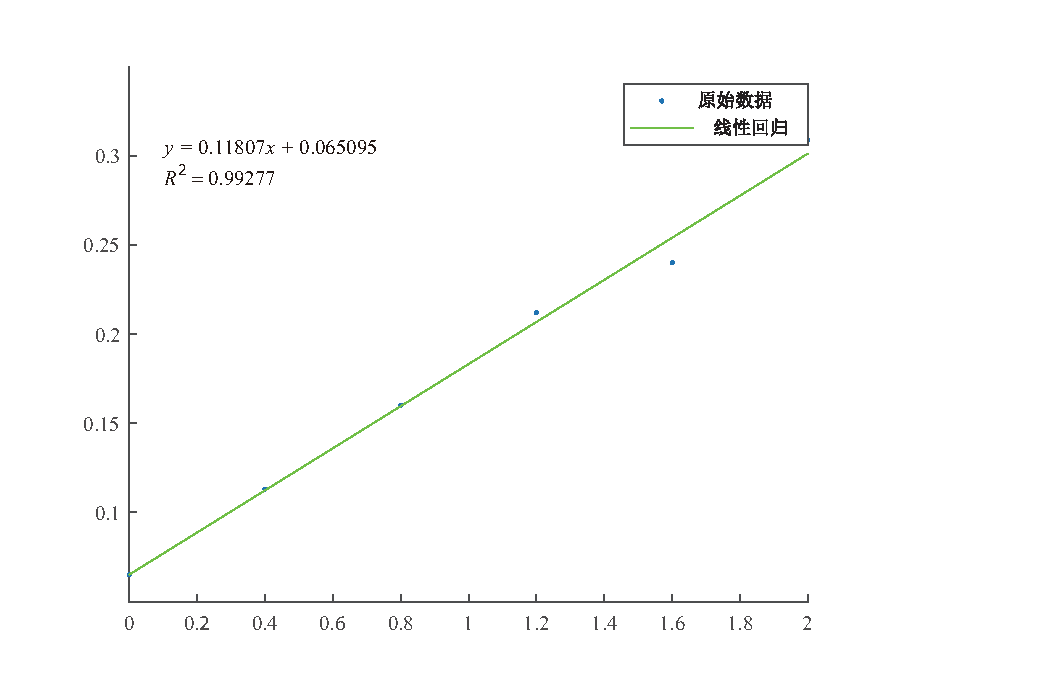
\includegraphics[width=8cm,height=4.944cm]{./src/fig1.eps}}
	\subfigure[先加入样品反应后的标准曲线]{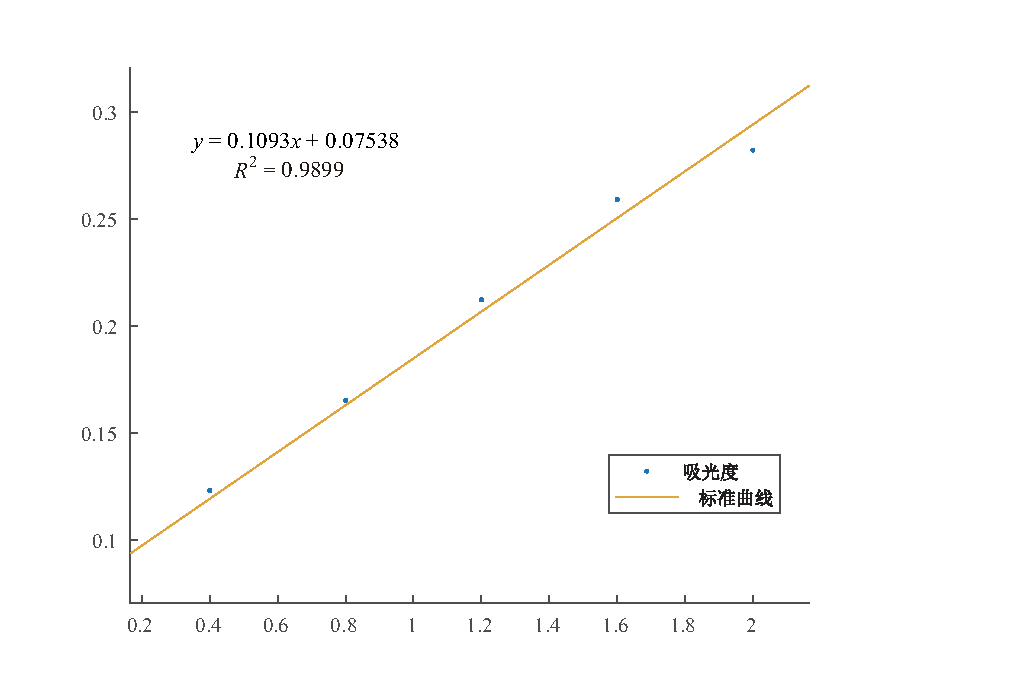
\includegraphics[width=8cm,height=4.944cm]{./src/fig2.eps}}
	\caption{两种方法获得的标准曲线}
\end{figure}
\subsection{实验数据}
% Please add the following required packages to your document preamble:
\begin{table}[htb]
	\center
	\caption{标准样品反应后吸光值}
	\setlength{\tabcolsep}{4cm}{
	\begin{tabular}{@{}cc@{}}
		\toprule
		先加入双缩脲试剂反应 & 先加入样品反应 \\ \midrule
		0.065      & 0.067   \\
		0.113      & 0.123   \\
		0.16       & 0.165   \\
		0.212      & 0.212   \\
		0.24       & 0.259   \\
		0.309      & 0.282   \\ \bottomrule
	\end{tabular}}
\end{table}
\begin{table}[htb]
	\center
	\caption{IgG样品吸光值和稀释血浆的总蛋白浓度}
	\setlength{\tabcolsep}{3cm}{
	\begin{tabular}{@{}cc@{}}
		\toprule
		IgG & 血浆总蛋白 \\ \midrule
		0.241      & 0.245   \\
		0.177      & 0.183   \\ \bottomrule
	\end{tabular}}
\end{table}
\begin{thebibliography}{99}
	\bibitem{ref1}{钱国正,汪丽曼.判别二个线性回归方程是否显著差异的统计方法[J].第二军医大学学报,1992(06):583-585.}
\end{thebibliography}
\end{document}